\section{Příklad 3}
% Jako parametr zadejte skupinu (A-H)
\tretiZadani{C}

\subsection{Uprava schemy}
Najskor si musime upravit schemu obvodu. Vsetky napatove zdroje musime nahradit za prudove a vsetky odpory musime nahradit za vodivosti.

\begin{figure}[!h]
    \centering
    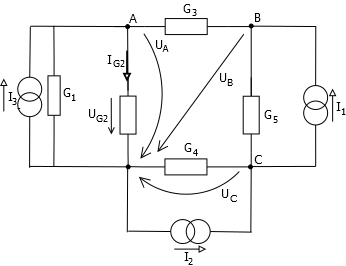
\includegraphics[width=0.5\linewidth]{pr3/1.png}
\end{figure}

\begin{align*}
    G_1 &= \frac{1}{R_1} = \frac{1}{44} S \\
    G_2 &= \frac{1}{R_2} = \frac{1}{31} S\\
    G_3 &= \frac{1}{R_3} = \frac{1}{56} S\\
    G_4 &= \frac{1}{R_4} = \frac{1}{20} S \\
    G_5 &= \frac{1}{R_5} = \frac{1}{30} S \\
    \\
    I_3 &= \frac{U}{R_1} = \frac{110}{44} == \SI{2.5}{\ampere}\\
\end{align*}

\subsection{Zostrojenie matice a vypocet $U_A$, $U_B$, $U_C$}
Teraz mozeme zostrojit maticu pre vypocet uzlovych napati.
Na hlavnu diagonalu dame sucet vsetkych vodivosti ktore su pripojene na dany uzol. 
Na zvysne pozicie data zaporne otoceny sucet vsetkych vodivosti ktore spajaju dane dva uzly.

\begin{figure}[!h]
    \centering
    \begin{equation}
    \begin{pmatrix}
    G_1 + G_2 + G_3  & -G_3 & 0\\
    -G_3  & G_3 + G_5 & -G_5\\
    0  & -G_5 & G_4+G_5 \\
    \end{pmatrix}
    \cdot
    \begin{pmatrix}
    U_A\\
    U_B\\
    U_C\\
    \end{pmatrix}
    =
    \begin{pmatrix}
    I_3\\
    I_1\\
    -I_1+I_2\\
    \end{pmatrix}
    \end{equation}
\end{figure}
\begin{figure}[!h]
    \centering
    \begin{equation}
    \begin{pmatrix}
    \frac{1}{44} S + \frac{1}{31} S +\frac{1}{56} S  & +\frac{1}{56} S & 0\\
    -\frac{1}{56} S  & \frac{1}{56} S + \frac{1}{30} S & -\frac{1}{30} S\\
    0  & -\frac{1}{30} S & \frac{1}{20} S+\frac{1}{30} S \\
    \end{pmatrix}
    \cdot
    \begin{pmatrix}
    U_A\\
    U_B\\
    U_C\\
    \end{pmatrix}
    =
    \begin{pmatrix}
    \SI{2.5}{\ampere}\\
    \SI{0.85}{\ampere}\\
    -\SI{0.85}{\ampere}+\SI{0.75}{\ampere}\\
    \end{pmatrix}
    \end{equation}
\end{figure}

\begin{align*}
    U_A &=  \SI{44.73937}{\volt}\\
    U_B &= \SI{42.49970}{\volt}\\
    U_C &= \SI{15.79988}{\volt}\\
\end{align*}

\subsection{Vypocet $U_{R2}$ a $I_{R2}$}
Napatie $U_A$ sa rovna $U_{R2}$ a preto staci ked dopocitame $I_{R2}$.

\begin{align*}
    I_{R2} = \frac{U_2}{R_2}  &= \frac{\SI{44.73937}{\volt}}{\SI{31}{\ohm}} = \SI{1.443205483}{\ampere}\\
\end{align*}